\documentclass[a4paper]{article}

%% Language and font encodings
\usepackage[english]{babel}
\usepackage[utf8x]{inputenc}
\usepackage[T1]{fontenc}

%% Sets page size and margins
\usepackage[a4paper,top=3cm,bottom=2cm,left=3cm,right=3cm,marginparwidth=1.75cm]{geometry}

%% Useful packages
\usepackage{amsmath}
\usepackage{graphicx}
\usepackage[colorinlistoftodos]{todonotes}
\usepackage[colorlinks=true, allcolors=blue]{hyperref}

\title{Evaluación 1: Análisis de las mareas y salinidad en el Manglar El Sargento.}
\author{Jesús Antonio González Espinosa \\ \\ Física Computacional 1}
\date{8 de Marzo del 2018}

\begin{document}
\maketitle

\section{Archivos}
Después de crear la carpeta Evaluación1,iniciamos la actividad descargando los dos archivos  de datos de El Sargento que vienen en la página del curso.
La instrucción indica que nos tenemos que asegurar que ambos archivos abarquen el mismo periodo de tiempo, entonces, con Emacs analizamos los datos para ver que tan desfasados estaban. Después de una rápida hojeada a los datos, se pudo observar que solo eran dos renglones los que causaban que los datos no estuvieran en el mismo periodo de tiempo: el primer renglón del archivo $sargento-salinidad-201117.csv$ y el último renglón de $sargento_201117$. Entonces para poder corregirlos, teníamos que deshacernos de esos dos, pero al saber que solo eran renglones a los extremos, se decidió dejarlo la corrección para después, ya que contamos con las herramientas necesarias en Pandas, para hacerlo más rápido. 


\section{Jupyter Notebook}
Lo que sigue de la actividad fue abrir $Jupyter Notebook$ en la carpeta de Evaluación1. Ahí, creamos un documento tipo notebook con Python 3. Ahí cargamos las biblotecas de Pandas, Numpy, datetime, matplotlib.pyplt y seaborn, las cuales son necesarias para hacer la actividad.  

\subsection{Lectura en Pandas}
Primero cargamos el archivo $sargento_201117.csv$ bajo el data frame de nombre $dfsargento1$, asegurándonos de saltarnos las dos primeros renglones del documento, que son texto innecesario, darle nombre a las columnas y hacer que ignore el último renglón, para que este coincida con el final del otro archivo. Asimismo, cargamos el otro archivo, $sargento-salinidad-201117.csv$ bajo el data frame $dfsargento2$, hacemos lo mismo, pero ahora saltando los tres primeros renglones, siendo uno de datos pero a una hora que no incluye el otro archivo; y finalmente le damos nombre a las columnas. Seguido a esto, se imprimió en la pantalla la tabla con los últimos datos para asegurarnos que ambos tengan la misma cantidad de renglones y que acaben a la misma hora:

\pagebreak
\begin{figure}[h!]
 \centering
  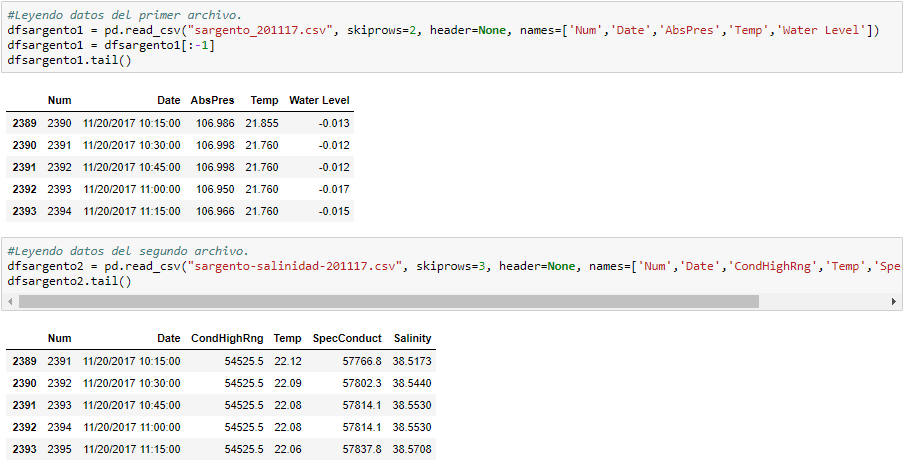
\includegraphics[width=0.8\textwidth]{datos1.PNG}
\end{figure}

Ahora, vimos el tipo de datos que son, para asegurar que todos sean variables, y se pudo notar que la fecha era de tipo objeto, pero gracias a la libereria datetime pudimos arreglar eso y crear dos nuevas columnas, una para todas las fechas, y otra para los meses. Finalmente, los datos están listos para ser utilizados y graficados.  

\begin{figure}[ht!]
 \centering
  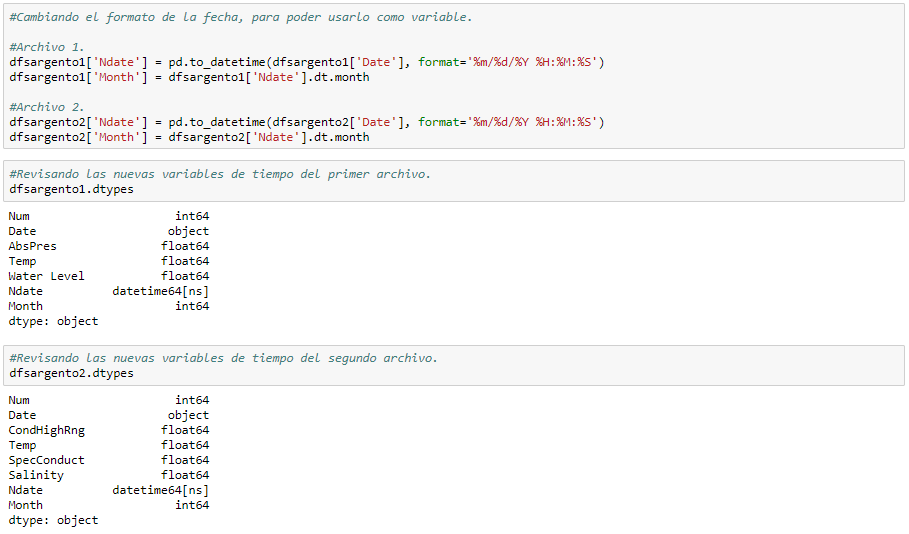
\includegraphics[width=0.8\textwidth]{datos2.PNG}
\end{figure}

\pagebreak
\subsection{Gráficas Seaborn}
Ahora, con ayuda de la librería Seaborn, vamos a graficar varios tipo de gráficas, para observar los datos. 
\subsubsection{Boxplot}
El primer tipo de gráfica es boxplot. Para cada dato que se grafique, se van a mostrar dos, una correspondiente a cada mes. El código utilizado fue:
\begin{figure}[h!]
 \centering
  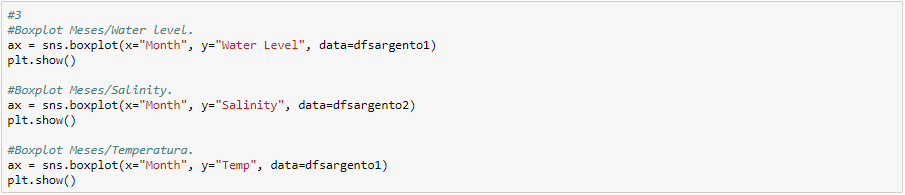
\includegraphics[width=0.8\textwidth]{BoxplotCodigo.PNG}
\end{figure}
Cada una creó las siguientes gráficas:

La primer es del Nivel del Mar:
\begin{figure}[ht!]
 \centering
  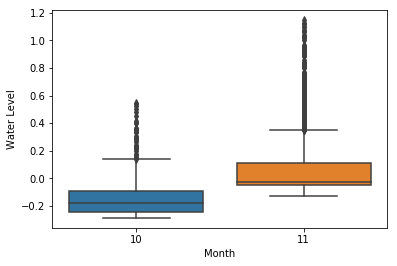
\includegraphics[width=0.6\textwidth]{Boxplot1.png}
\end{figure}

El siguiente boxplot es de Salinidad:
\begin{figure}[ht!]
 \centering
  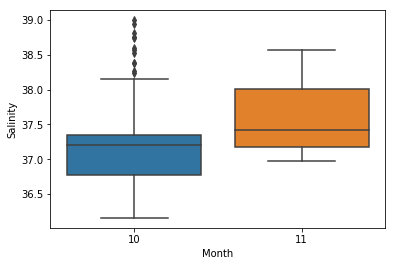
\includegraphics[width=0.6\textwidth]{Boxplot2.png}
\end{figure}

\pagebreak
El último de lox boxplot es de la Temperatura del Agua:
\begin{figure}[ht!]
 \centering
  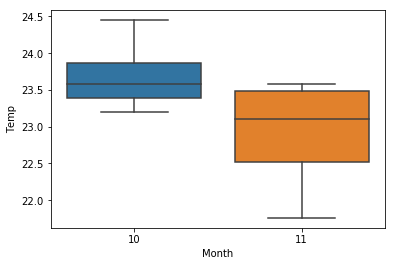
\includegraphics[width=0.6\textwidth]{Boxplot3.png}
\end{figure}

También podemos mostrar más información con la función $describe$, que muestra la posición de la mediana, los cuarteles, los máximos y mínimos. 
\begin{figure}[ht!]
 \centering
  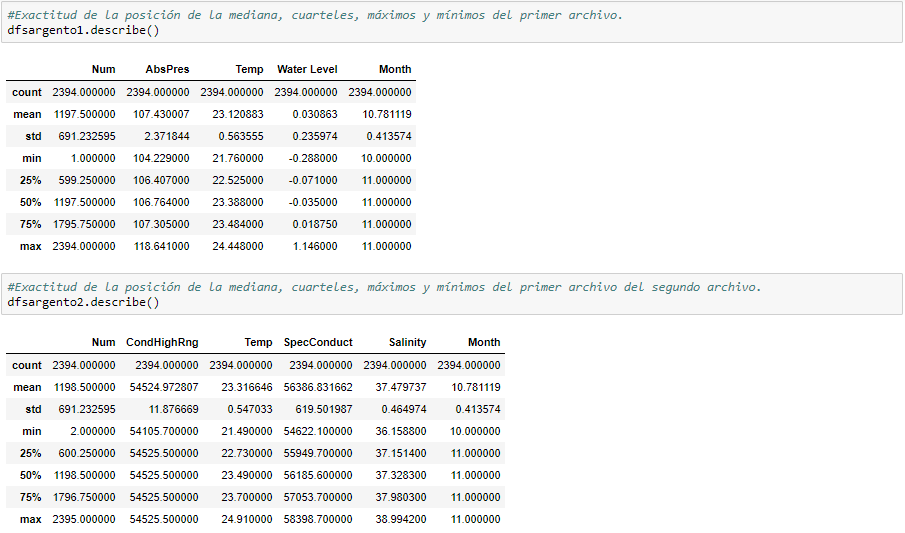
\includegraphics[width=0.7\textwidth]{Describe.PNG}
\end{figure}

\pagebreak
\subsubsection{Correlación de Pearson}
El segundo tipo de gráficas que se hacen son de Correlación de Pearson, en la que se graficaron parejas de variables. El código utilizado fue:
\begin{figure}[ht!]
 \centering
  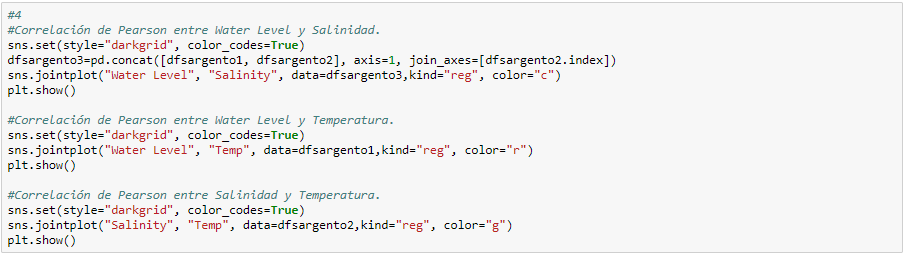
\includegraphics[width=0.8\textwidth]{PearsonCodigo.PNG}
\end{figure}
Cada una creó las siguientes gráficas:

El primer par de datos son Nivel de Mar - Salinidad:
\begin{figure}[ht!]
 \centering
  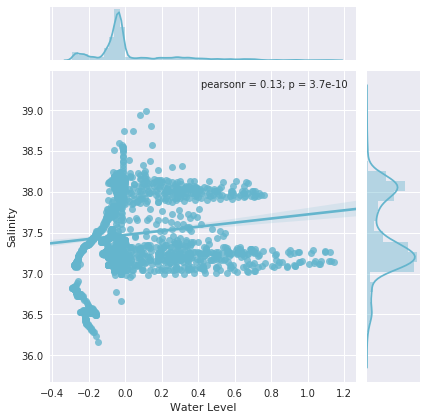
\includegraphics[width=0.6\textwidth]{Pearson1.png}
\end{figure}

El siguiente es Nivel de Mar - Temperatura de Agua:
\begin{figure}[ht!]
 \centering
  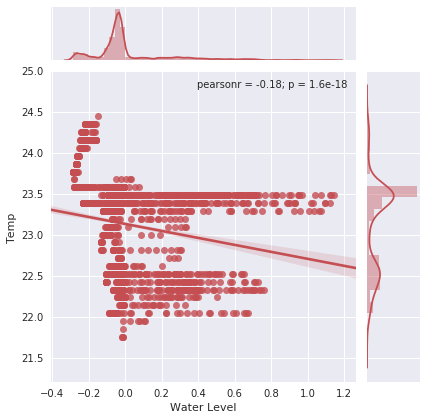
\includegraphics[width=0.6\textwidth]{Pearson2.png}
\end{figure}

\pagebreak
Finalmente tenemos Salinidad - Temperatura del Agua:
\begin{figure}[ht!]
 \centering
  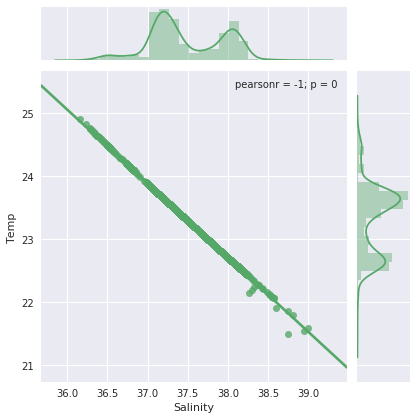
\includegraphics[width=0.6\textwidth]{Pearson3.png}
\end{figure}

Con esto, terminamos las gráficas de Seaborn.

\pagebreak
\subsection{Gráficas Matplotlib}
Ahora, empezamos a usar la librería Matplotlib para gráficar.
\subsubsection{Gráficas Independientes}
Aquí se usó la bibloteca matplotlib para graficar datos en función del tiempo. El código utilizado fue:
\begin{figure}[ht!]
 \centering
  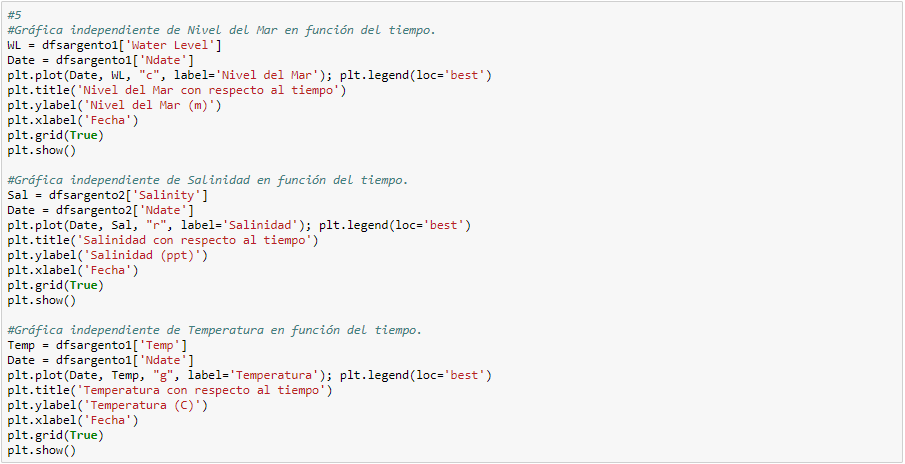
\includegraphics[width=0.6\textwidth]{IndeCodigo.PNG}
\end{figure}
Los cuales forman las siguientes gráficas: 

La primera es del Nivel del Mar como función del tiempo: 
\begin{figure}[ht!]
 \centering
  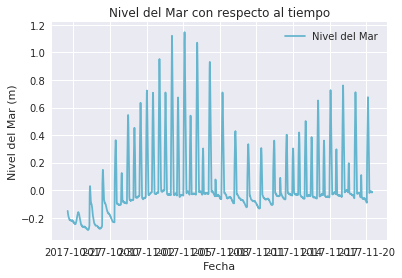
\includegraphics[width=0.8\textwidth]{Matplotlib1.png}
\end{figure}

La siguiente es de Salinidad como función del tiempo:
\begin{figure}[ht!]
 \centering
  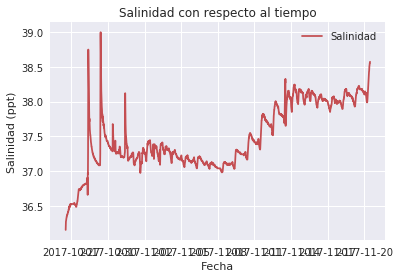
\includegraphics[width=0.6\textwidth]{Matplotlib2.png}
\end{figure}

\pagebreak
La última gráfica creada fue de Temperatura del Agua como función del tiempo:
\begin{figure}[ht!]
 \centering
  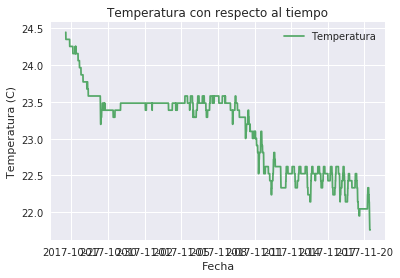
\includegraphics[width=0.6\textwidth]{Matplotlib3.png}
\end{figure}

\subsubsection{Gráficas con doble Eje}
De nuevo, utilizando Matplotlib se generaron gráficas superpuestas con doble eje vertical. Para estas se hizo el siguiente código:
\begin{figure}[ht!]
 \centering
  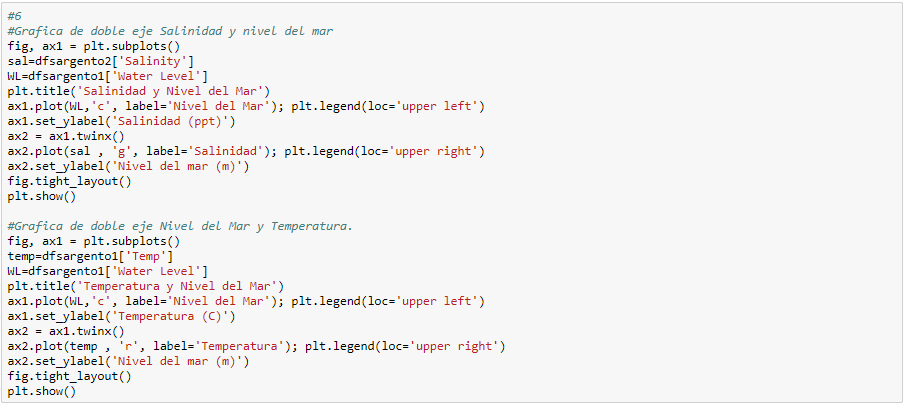
\includegraphics[width=0.8\textwidth]{DobleejeCodigo.PNG}
\end{figure}

El cual creó las siguientes gráficas:

\pagebreak
La primera es de Nivel del Mar y Salinidad:
\begin{figure}[ht!]
 \centering
  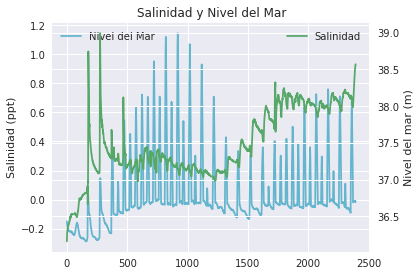
\includegraphics[width=0.6\textwidth]{Matplotlib4.png}
\end{figure}

Y la segunda, y última, es de Nivel de Mar y Temperatura:
\begin{figure}[ht!]
 \centering
  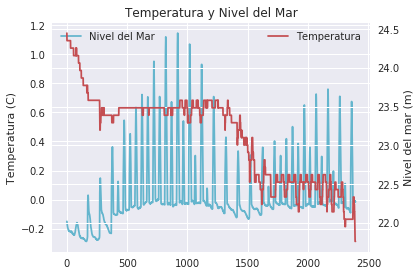
\includegraphics[width=0.6\textwidth]{Matplotlib5.png}
\end{figure}

\subsubsection{Gráficas con doble Eje con xlim}
Ahora, de nuevo repetimos el código y proceso de las últimas dos gráficas, pero vamos a hacer que avancen en función del tiempo y vamos a usar la función xlim, para limitar las imágenes de las gráficas a cinco días. El código modificado a las especificaciones nuevas fue:
\begin{figure}[ht!]
 \centering
  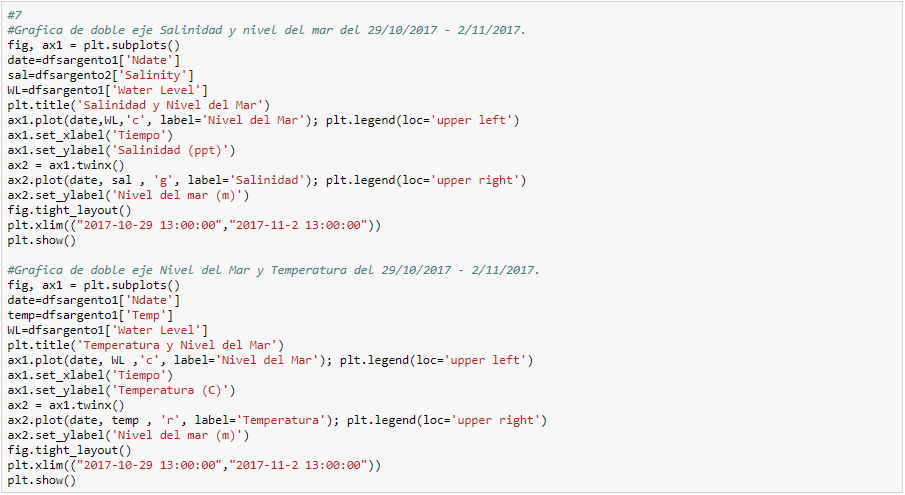
\includegraphics[width=0.8\textwidth]{DoblexLimCodigo.PNG}
\end{figure}

El cual creó las siguientes gráficas:

\pagebreak
La primera, Salinidad y Nivel del Mar en función del tiempo, del día 29/10/2017, hasta el día 2/11/2017:
\begin{figure}[ht!]
 \centering
  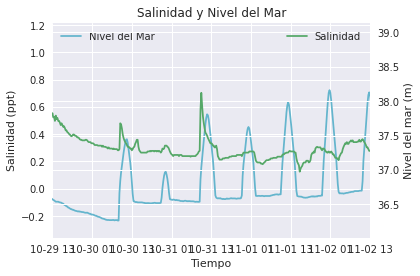
\includegraphics[width=0.6\textwidth]{Matplotlib6.png}
\end{figure}

La última gráfica de esta parte y toda la actividad, que es del Nivel del Mar y la Temperatura en función del tiempo, del día 29/10/2017, hasta el día 2/11/2017:
\begin{figure}[ht!]
 \centering
  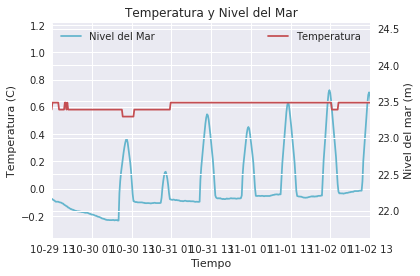
\includegraphics[width=0.6\textwidth]{Matplotlib7.png}
\end{figure}

Al ver las gráficas, podemos observar que en la de la Salinindad y el Nivel del Mar sí parece haber ciertos indicios de una relación, ya que en la primera mitad de la gráfica parece mostrar que si una aumenta, la otra también parece aumentar, pero en la siguiente mitad, parece hacer lo contrario. Por lo tanto, podemos decir que sí parece existir una relación entre los datos, solo que esta no es muy aparente.
Por otra parte, en la gráfica de Temperatura y Nivel del Mar no parece haber relación alguna entre los datos. 

\bigskip
\section{Conclusión}
Fue interesante trabajar en esta evaluación, ya que por una parte trabajamos con datos locales, lo cual a mi parecer es muy interesante, y por otro lado, porque unificamos todas las herramientas que adquirimos en lo que lleva el curso. Otro factor importante fue el hecho de que la evaluación fue como hacer una actividad pero contrarreloj, lo que lo hizo parecer como un reto, que a mi parecer lo hizo divertido. Al final de cuentas, el tiempo sí fue suficiente, y el trabajo realizado se ha sentido satisfactorio. 


\end{document}